%%%%%%%%%%%%%%%%%%%%%%%%%%%%%%%%%%%%%%%%%
% Stylish Article
% LaTeX Template
% Version 2.1 (1/10/15)
%
% This template has been downloaded from:
% http://www.LaTeXTemplates.com
%
% Original author:
% Mathias Legrand (legrand.mathias@gmail.com) 
% With extensive modifications by:
% Vel (vel@latextemplates.com)
%
% License:
% CC BY-NC-SA 3.0 (http://creativecommons.org/licenses/by-nc-sa/3.0/)
%
%%%%%%%%%%%%%%%%%%%%%%%%%%%%%%%%%%%%%%%%%

%----------------------------------------------------------------------------------------
%	PACKAGES AND OTHER DOCUMENT CONFIGURATIONS
%----------------------------------------------------------------------------------------

\documentclass[fleqn,10pt]{SelfArx} % Document font size and equations flushed left

\usepackage[italian]{babel} % Specify a different language here - english by default

\usepackage{float}
%----------------------------------------------------------------------------------------
%	COLUMNS
%----------------------------------------------------------------------------------------

\setlength{\columnsep}{0.55cm} % Distance between the two columns of text
\setlength{\fboxrule}{0.75pt} % Width of the border around the abstract

%----------------------------------------------------------------------------------------
%	COLORS
%----------------------------------------------------------------------------------------

\definecolor{color1}{RGB}{0,0,90} % Color of the article title and sections
\definecolor{color2}{RGB}{0,20,20} % Color of the boxes behind the abstract and headings

%----------------------------------------------------------------------------------------
%	HYPERLINKS
%----------------------------------------------------------------------------------------

\usepackage{hyperref} % Required for hyperlinks
\hypersetup{hidelinks,colorlinks,breaklinks=true,urlcolor=color2,citecolor=color1,linkcolor=color1,bookmarksopen=false,pdftitle={Title},pdfauthor={Author}}

%----------------------------------------------------------------------------------------
%	ARTICLE INFORMATION
%----------------------------------------------------------------------------------------

\JournalInfo{Progetto di \textit{Foundation of Probability and Statistics}, Università degli Studi di Milano Bicocca} % Journal information
\Archive{Anno Accademico 2019-20} % Additional notes (e.g. copyright, DOI, review/research article)

\PaperTitle{Spotify Dataset - Analisi delle tracce musicali e previsione della popolarità} % Article title

\Authors{Riccardo Cervero\textsuperscript{1}} % Authors
\affiliation{\textsuperscript{1}\textit{794126, Dipartimento di Informatica, Sistemistica e Comunicazione}} % Author affiliation

\Keywords{Inferenza - Previsione} 
\newcommand{\keywordname}{Keywords} 

%----------------------------------------------------------------------------------------
%	ABSTRACT
%----------------------------------------------------------------------------------------

\Abstract{Durante l'ultimo ventennio, grazie allo sviluppo di applicazioni \textit{web} per l'ascolto sempre più efficienti, la fruizione di contenuti musicali ha mostrato un'importante e rapida evoluzione, permettendo all'utente di accedere a qualsiasi brano - o qualunque versione dello stesso - in brevissimo tempo e, nella maggior parte dei casi, gestire autonomamente un archivio di tracce e artisti preferiti. L'industria discografica ha saputo sfruttare tale progresso, non soltanto incrementando il volume di distribuzione e di campagne promozionali, ma anche approfondendo quantitativamente e qualitativamente le tendenze d'ascolto di un pubblico catalogato. Moderne piattaforme offrono, infatti, la possibilità di estrarre ed analizzare una vasta varietà di parametri acustici e non, cosicché il produttore possa dedurre quali sono le caratteristiche più ricercate dal pubblico in un determinato momento e aumentare così la popolarità della traccia. È il caso, ad esempio, di \textit{Spotify}. Questo progetto, pertanto, ha come obiettivo l'analisi statistica delle caratteristiche qualitative e quantitative registrate da \textit{Spotify} in un \textit{database} di tracce disponibili all'interno del proprio servizio di \textit{streaming musicale}. Più precisamente, nella seconda e terza sezione verranno esaminate le variabili,  testata la loro reciproca connessione - di tipo lineare o non - e calcolate stime intervallari per le rispettive medie o proporzioni fra le modalità. Infine, nelle due successive sezioni, verranno esposti i risultati dei modelli di regressione lineare - sia semplice che multivariata - per la previsione della popolarità del brano e della positività emotiva da esso trasmessa.} 

%----------------------------------------------------------------------------------------

\begin{document}

\flushbottom % Makes all text pages the same height

\maketitle % Print the title and abstract box

\tableofcontents % Print the contents section

\thispagestyle{empty} % Removes page numbering from the first page

%----------------------------------------------------------------------------------------
%	ARTICLE CONTENTS
%----------------------------------------------------------------------------------------

\section{Caso di studio}
I dati esaminati nell'ambito di questo progetto provengono dal database di \textit{Kaggle} "Spotify Dataset"\footnote{Il link da cui è possibile scaricare il database "Spotify Dataset" è \href{https://www.kaggle.com/yamaerenay/spotify-dataset-19212020-160k-tracks}{\texttt{/kaggle/spotify-dataset-160k-tracks}}.}, che raccoglie un totale di 19 caratteristiche acustiche e qualitative relative a 169909 tracce, rese disponibili sulla piattaforma \textit{Spotify for Developers}.\footnote{La documentazione della piattaforma \textit{Spotify for Developers} è disponibile al link \href{https://developer.spotify.com}{\texttt{developer.spotify.com}}.}\\
Le variabili oggetto di studio\footnote{La descrizione ufficiale delle variabili è disponibile ai link \href{https://developer.spotify.com/documentation/web-api/reference/tracks/get-audio-features/}{\texttt{developer.spotify/audio-features}} e \href{https://developer.spotify.com/documentation/web-api/reference/tracks/get-track/}{\texttt{developer.spotify/get-track}}.} corrispondono alle seguenti grandezze:
\begin{itemize}
    \item \textit{Acousticness} - o "acusticità" , è misura numerica - fra 0 e 1 - della confidenza con cui è possibile definire "acustica" una traccia: se 1, indica massima certezza nell'affermare che il brano sia stato prodotto senza strumenti elettronici
    \item \textit{Danceability} è il grado di ballabilità calcolato fra 0 e 1, come combinazione di vari elementi musicali, fra cui la stabilità del ritmo e il tempo
    \item \textit{Duration} è la durata del brano in millisecondi
    \item \textit{Energy} rappresenta la percentuale di intensità della traccia, sulla base di elementi percettivi quali sonorità e timbro
    \item \textit{Explicit} è variabile binaria che rileva la presenza o meno di contenuto esplicito
    \item \textit{Instrumentalness} misura, fra 0 e 1, l'assenza di contenuto vocale: più il valore si avvicina a 1, maggiore è la confidenza con cui si definisce "strumentale" la traccia
    \item \textit{Key} registra la stima della chiave complessiva della traccia, codificata in un valore numerico compreso fra 0 (Do) e 11 (Si)
    \item \textit{Liveness} rileva la presenza di un pubblico udibile nella registrazione, definendone la probabilità: se superiore a 0,8, fornisce una forte evidenza che la traccia sia stata registrata dal vivo
    \item \textit{Loudness} è il volume complessivo in decibel, fra -60 e circa 4
    \item \textit{Mode} è la variabile binaria circa la tonalità del brano: 1 se maggiore, 0 se minore
    \item \textit{Speechiness} indica la presenza di parlato: maggiore la somiglianza tra la traccia e un discorso - come nel caso del genere \textit{rap} -, maggiore la vicinanza del valore a 1
    \item \textit{Tempo} è il ritmo misurato in battiti al minuto (bpm)
    \item \textit{Valence} definisce il grado di positività emotiva trasmessa dal brano, tra 0 e 1
    \item \textit{Year} è l'anno di uscita del brano, dal 1921 al 2020
    \item \textit{Popularity} è una variabile intera compresa fra 0 e 100, che esprime il grado di popolarità del brano, calcolato a partire dal numero totale di riproduzioni su \textit{Spotify} e da quanto sono recenti tali ascolti: in generale, tracce riprodotte molto frequente durante l'anno corrente avranno un valore di popolarità molto elevato
\end{itemize}
Tali colonne verranno presentate singolarmente nei diversi paragrafi delle Sezioni \ref{cqual} e \ref{cquant}. In particolare, la popolarità verrà considerata come principale variabile \textit{target} nell'ambito della definizione di modelli di regressione.\\
\subsection{Pre-processing}
Il dataset originale non presentava alcun valore mancante, e le uniche operazioni di \textit{pre-processing} hanno implicato il raggruppamento delle modalità dell'anno di pubblicazione in classi di decennio (Sezione \ref{year}) e la rimozione delle variabili poco interessanti per l'obiettivo di analisi statistica: l'identificatore primario della traccia, il titolo, la lista di artisti accreditati e la data di pubblicazione. In particolare, la data di pubblicazione \textit{Release\_date} si manifestava in formato YYYY-MM-DD soltanto nel 70\% dei casi, mentre la restante parte riportava soltanto l'anno, così come la colonna \textit{Year}. Non potendo risalire al mese e al giorno, si è preferito eliminare \textit{Release\_date}.
%------------------------------------------------
\section{Analisi dei caratteri qualitativi}\label{cqual}
\subsection*{Variabile \textit{Year}}\label{year}
Le osservazioni del database "Spotify Dataset" sono distribuite con una certa coerenza fra i singoli anni - dal 1921 al 2020: le frequenze relative delle modalità di \textit{Year} sono identiche o comunque molto simili a 0.012 - che corrisponde alla frequenza relativa massima - in 73 anni su 100. Osservazioni meno numerose sono comprensibilmente relative agni anni precedenti al 1947. Perciò, la distribuzione di questa variabile qualitativa ordinale, oltre ad essere multimodale, può anche essere definita estremamente eterogenea: infatti, la mutabilità del fenomeno, misurata dall'indice normalizzato di Gini, mostra un valore di 0.999.\\
Poichè è noto che le tendenze musicali possono essere meglio definite nell'arco di decadi, piuttosto che di singole stagioni, si è deciso di aggregare le osservazioni per decenni. Le rispettive frequenze delle decadi sono intuibili in Figura \ref{fig:fig1}. 
\begin{figure}[H]
    \centering
    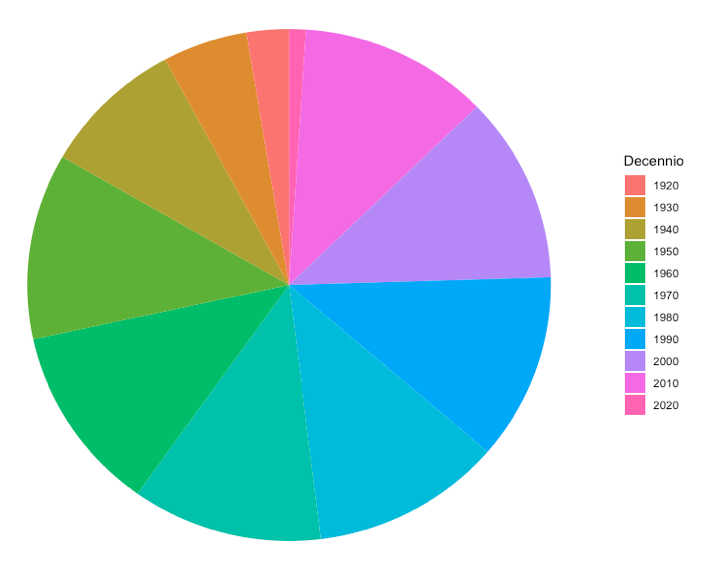
\includegraphics[width=0.7 \linewidth]{fig1.png}
    \label{fig:fig1}
    \caption{Aerogramma per la visualizzazione delle frequenze relative dei decenni.}
\end{figure}
Si è poi proceduto a verificare l'esistenza di una connessione fra questa nuova variabile e il grado di popolarità dei brani, eseguendo un test Chi-quadrato, cui ipotesi nulla
\begin{equation}
  H_0:\chi^2=0  
\end{equation}
coincide con l'indipendenza fra i due fenomeni. L'indice di associazione $\chi^2$ è dunque calcolato con $(k_1-1)(k_2-1)=990$ gradi di libertà, con $k_1=11$ e $k_2=100$ i rispettivi conteggi delle modalità. Fissato un livello di significatività $\alpha=0.05$, è stato ottenuto un valore \textit{pvalue} considerevolmente inferiore ad $\alpha$\footnote{Il \textit{pvalue} in questione è inferiore alla soglia $2.2\bullet10^{-16}$.}, portando a rifiutare, con confidenza al 95\%, l'ipotesi nulla di indipendenza fra il decennio di uscita della traccia e il proprio grado di popolarità. Ciò significa che le distribuzioni condizionali della popolarità variano in base alla decade considerata, come visibile in Figura \ref{fig:fig2}. 
\begin{figure}[H]
    \centering
    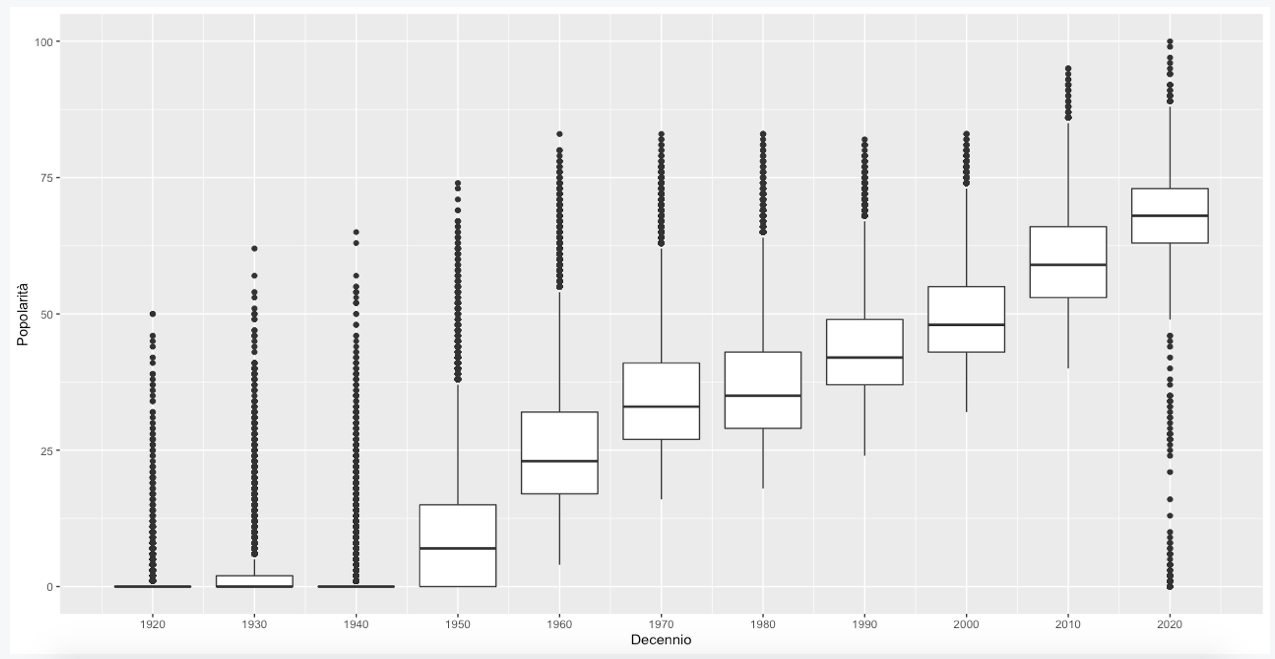
\includegraphics[width=1 \linewidth]{fig2.png}
    \label{fig:fig2}
    \caption{\textit{BoxPlot} condizionati per la visualizzazione delle distribuzioni condizionate di popolarità in base al decennio esaminato.}
\end{figure}
La natura di questa dipendenza statistica viene approfondita mediante test ANOVA, basato sull'ipotesi nulla di uguaglianza di tutte le popolarità medie, ovvero sull'ipotesi che le osservazioni di popolarità relative a ciascun decennio provengano da popolazioni che seguono una distribuzione normale con varianza e media pari. Si punta pertanto a verificare l'ipotesi alternativa, cioè che la media di almeno un gruppo differisca dalle altre, dimostrando che il fattore condizionante della decade ha un'influenza sulla popolarità. La statistica test è associata a 10 gradi di libertà e, fissato un livello di significatività $\alpha=0.05$, è stato ottenuto un valore \textit{pvalue} ancora una volta nettamente inferiore ad $\alpha$, causando il rifiuto dell'ipotesi nulla di uguaglianza delle popolarità medie per decennio e confermando, con una confidenza al 95\%, la presenza di una forte relazione fra queste due variabili. Osservando la Figura, è possibile riscontrare, almeno visivamente, una tendenza comprensibile: la preferenza degli utenti a livello aggregato appare quasi perfettamente ordinata per "novità" del brano.

\subsection*{Variabile \textit{Explicit}}
Un fenomeno, al contrario, distribuito in maniera poco equilibrata è la presenza di contenuto esplicito nel testo: la frequenza percentuale delle tracce non esplicite è pari al 91.51\% (Figura \ref{fig:fig3}) e il suo indice di Gini normalizzato conferma la bassa mutabilità: $\sim$0.311. 
\begin{figure}[H]
    \centering
    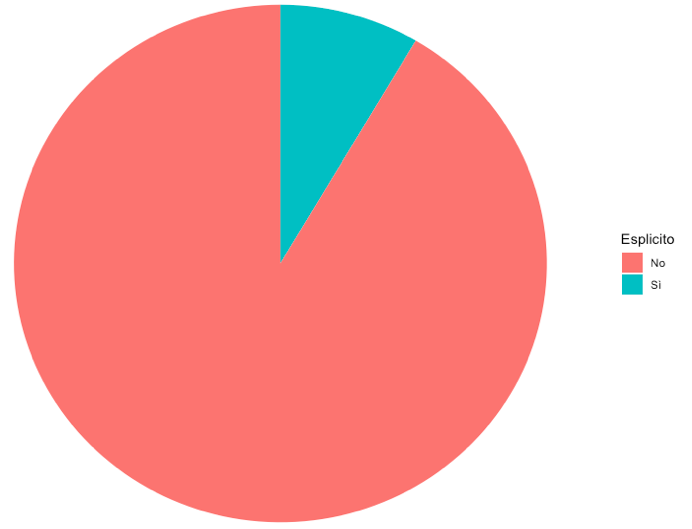
\includegraphics[width=0.7 \linewidth]{fig3.png}
    \label{fig:fig3}
    \caption{Aerogramma per la visualizzazione delle rispettive frequenze relative di contenuto esplicito e non esplicito.}
\end{figure}
Nonostante l'elevata numerosità del campione studiato, rimane più utile e affidabile la pratica di stima intervallare del parametro di proporzione $p$, che deriva dallo studio della distribuzione campionaria della frequenza relativa di una determinata classe nella popolazione. L'intervallo di confidenza ottenuto, avrà pertanto i seguenti estremi:
\begin{equation}
    (p-z_{\frac{\alpha}{2}}\sqrt{\frac{p(1-p)}{n}};p+z_{\frac{\alpha}{2}}\sqrt{\frac{p(1-p)}{n}})
\end{equation}
In questo caso, fissato un livello di significatività $\alpha=0.05$, i rispettivi intervalli di confidenza delle modalità "esplicito" e "non esplicito" - con estremi approssimati al terzo decimale - sono:
\begin{equation}
    (0.084, 0.086)\\(0.914, 0.916)
\end{equation}
Anche in questo caso, viene verificata l'esistenza di una connessione fra il grado di popolarità e la presenza di contenuto esplicito: ad un livello di confidenza del 95\% e con 99 gradi di libertà, l'ipotesi di indipendenza fra le due variabili viene rifiutata poiché il \textit{pvalue} è calcolato nettamente inferiore alla soglia di significatività.\\
Inoltre, eseguendo un test ANOVA sull'uguaglianza delle due popolarità medie in corrispondenza di contenuto esplicito e non esplicito, si ottiene un \textit{pvalue} molto basso, rifiutando nuovamente l'ipotesi nulla con un livello di confidenza al 95\%.
\begin{figure}[H]
    \centering
    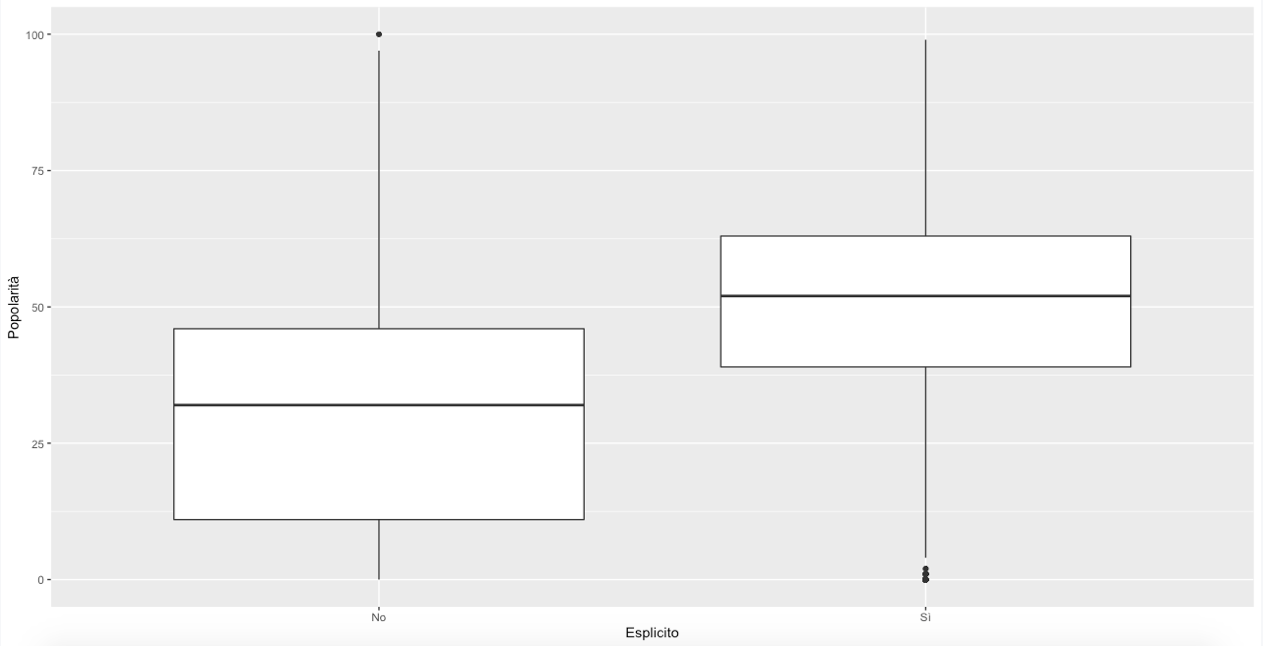
\includegraphics[width=1 \linewidth]{fig4.png}
    \label{fig:fig4}
    \caption{\textit{BoxPlot} condizionati per la visualizzazione delle distribuzioni condizionate di popolarità in base alla presenza o meno di contenuto esplicito.}
\end{figure}

\subsection*{Variabile \textit{Mode}}
La distribuzione delle due tonalità si presenta sbilanciata: la frequenza percentuale della modalità "maggiore" è circa il 70.9\%, contro il 29.1\% della "minore" (Figura \ref{fig:fig5}).
\begin{figure}[H]
    \centering
    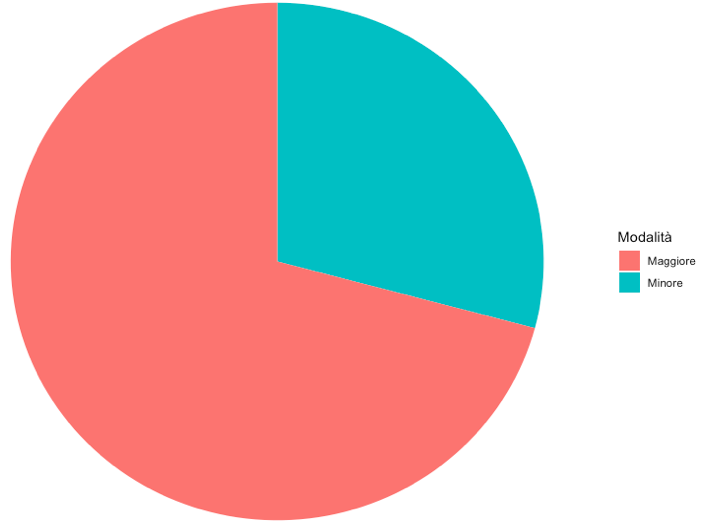
\includegraphics[width=0.7 \linewidth]{fig5.png}
    \label{fig:fig5}
    \caption{Aerogramma per la visualizzazione delle frequenze relative delle due tonalità.}
\end{figure}
L'indice di Gini normalizzato viene calcolato pari a 0.83.\\
Si è proceduto dunque ad estrarre un'informazione più accurata e affidabile tramite stima intervallare delle proporzioni di tracce in tonalità minore e maggiore nella popolazione: ad un livello di confidenza del 95\%, le rispettive probabilità sono contenute nei seguenti intervalli di confidenza - con estremi approssimati al terzo decimale:
\begin{equation}
    (0.289, 0.294)\\(0.706, 0.711)
\end{equation}
Viene rifiutata, ad un livello di confidenza del 95\%, l'ipotesi che l'indice di connessione $\chi^2$ per l'individuazione di una dipendenza statistica fra la tonalità del brano e la sua popolarità, calcolato con 99 gradi di libertà, sia nullo: il \textit{pvalue} ha un valore estremamente basso. Per lo stesso motivo, si rifiuta, tramite test ANOVA con $\alpha=0.05$, l'uguaglianza delle popolarità medie delle tracce condizionate alle due diverse tonalità.
\begin{figure}[H]
    \centering
    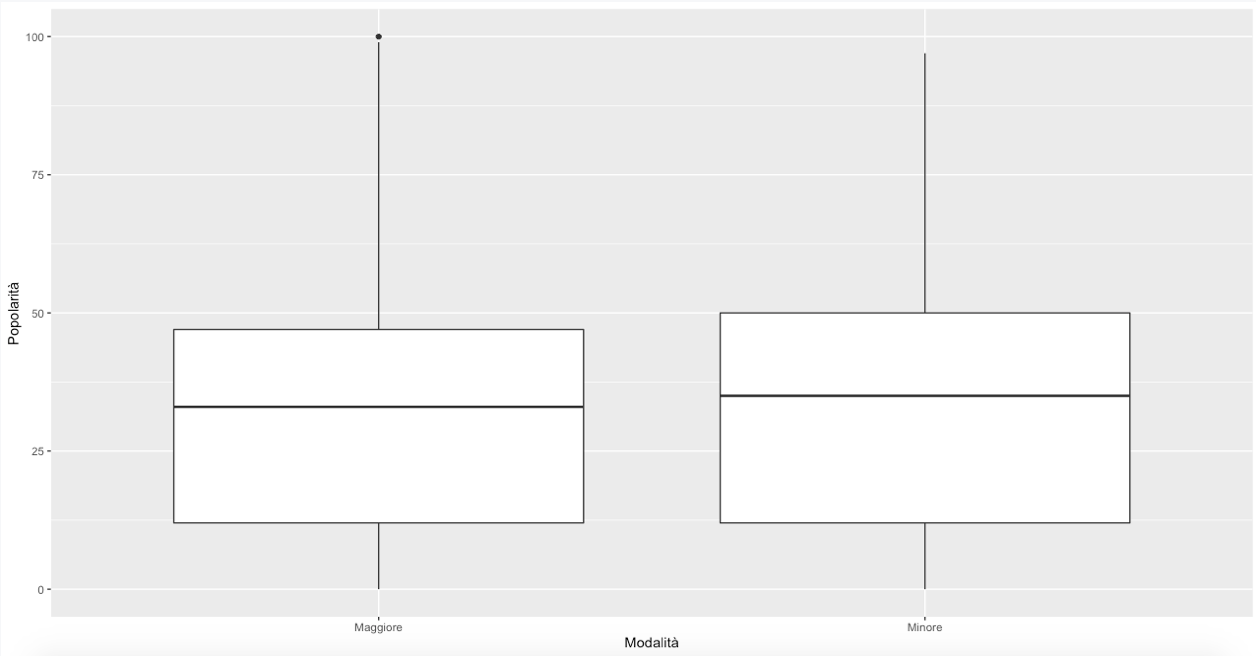
\includegraphics[width=1 \linewidth]{fig6.png}
    \label{fig:fig6}
    \caption{\textit{BoxPlot} condizionati per la visualizzazione delle distribuzioni condizionate di popolarità in base alla tonalità.}
\end{figure}

\subsection*{Variabile \textit{Key}}
L'ultimo carattere qualitativo, riferito alla chiave globale della traccia, mostra un'elevatissima eterogeneità: l'indice normalizzato di Gini è infatti pari a 0.991. È possibile, fra le 11 modalità, individuarne la moda: la chiave di "Do", con una frequenza percentuale del 12.65\%. Tuttavia, per poter affermare con più affidabilità che la chiave più frequente fra i brani musicali sia effettivamente "Do", è necessario confrontare le rispettive stime intervallari delle frequenze relative di tutte le modalità di \textit{Key}. Il risultato di ogni stima è riassunto in Figura \ref{fig:fig8}. Poiché gli estremi superiori degli intervalli di confidenza delle altre chiavi sono sempre minori rispetto al limite inferiore dell'intervallo di confidenza di "Do", è possibile affermare con un livello di confidenza del 95\% che essa sia, in effetti, la chiave più usata per comporre una traccia. Allo stesso modo, "Re diesis" può essere considerata come la chiave meno utilizzata.
\begin{figure}[H]
    \centering
    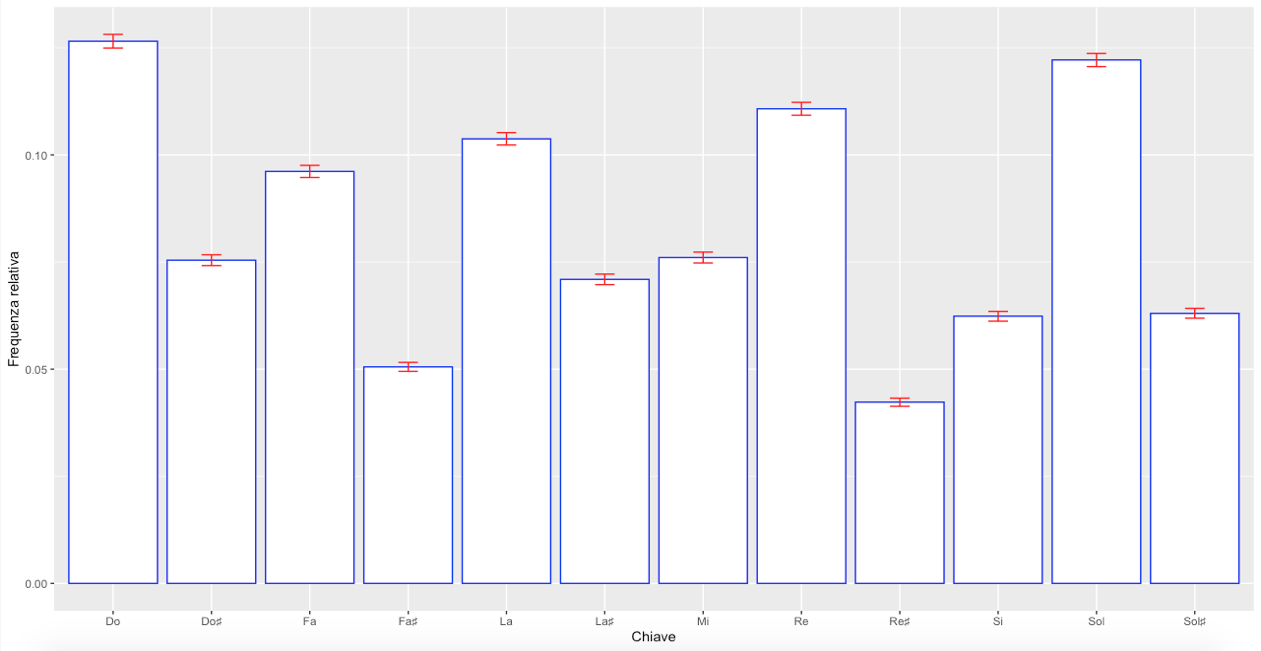
\includegraphics[width=1 \linewidth]{fig8.png}
    \label{fig:fig8}
    \caption{\textit{BarPlot} delle frequenze relative di ciascuna chiave nella popolazione. I segmenti rossi verticali indicano gli intervalli di confidenza calcolati con $(1-\alpha)=0.95$. Dall'osservazione del grafico, è possibile dedurre che "Do" sia la chiave più frequente.}
\end{figure}
Viene poi rifiutata, con un livello di significatività $\alpha=0.05$, l'ipotesi di indipendenza statistica fra la popolarità e la chiave. Infine, eseguendo un test ANOVA con livello di confidenza del 95\%, si rifiuta anche l'ipotesi di uguaglianza fra le popolarità medie condizionate alla chiave globale con cui è stata composta la traccia. Ciò significa che la scelta della chiave, così come la selezione di una determinata tonalità e l'introduzione di contenuto esplicito nel testo, ha un'influenza sul livello di popolarità che raggiungerà il brano.\\
In Figura \ref{fig:fig9}, è possibile osservare le distribuzioni della popolarità condizionata alla chiave.
\begin{figure}[H]
    \centering
    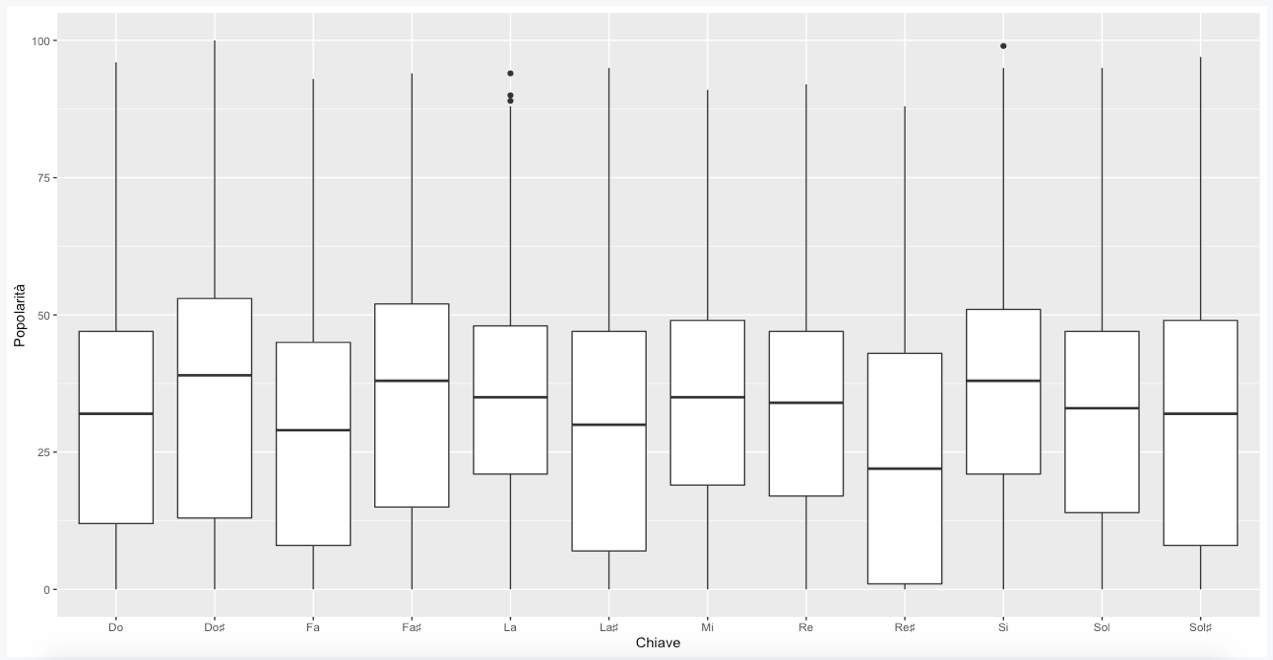
\includegraphics[width=1 \linewidth]{fig9.png}
    \label{fig:fig9}
    \caption{\textit{BoxPlot} condizionati per la visualizzazione delle distribuzioni condizionate di popolarità in base alla chiave globale.}
\end{figure}
%------------------------------------------------
\section{Analisi dei caratteri quantitativi}\label{cquant}
Tutte le rimanenti 11 variabili quantitative sono state esaminate in varie fasi:
\begin{itemize}
    \item calcolo delle statistiche descrittive di base, tra cui i principali momenti e quantili
    \item analisi della forma della distribuzione e confronto con una Normale
    \item stima intervallare della media della variabile - sempre con un livello di significatività $\alpha=0.05$ -, poiché, come già esposto per quanto riguarda la proporzione campionaria delle modalità qualitative, la sola stima puntuale derivata dal campione è dominata da una certa incertezza e mostra scarsa utilità
    \item analisi della significatività delle reciproche correlazioni lineari
\end{itemize}
Per evitare una descrizione prolissa del lavoro svolto, in questa Sezione verranno esposti soltanto i risultati riscontrati sulle variabili più interessanti.
\subsection*{Variabile \textit{Acousticness}}
Le statistiche descrittive sul livello di "acusticità" della traccia sono riassunte nella Tabella 1:
{\begin{table}[H]
\centering

\begin{tabular}[t]{lc}
\toprule
\midrule
\textbf{Minimo}&0\\
\textbf{1o Quartile}&0.0945\\
\textbf{Mediana}&0.492\\
\textbf{Media}&0.493\\
\textbf{3o Quartile}&0.888\\
\textbf{Massimo}&0.996\\
\textbf{Moda}&0.995\\
\textbf{Coeff. di Variazione}&0.764\\
\bottomrule
\end{tabular}
\caption{Statistiche descrittive calcolate sul livello di acusticità.}
\end{table}}
Dal fatto che moda e mediana differiscano è possibile dedurre che la distribuzione sia asimmetrica. Tuttavia, la differenza quasi trascurabile fra di esse è indizio di uno scarso grado di deviazione dalla condizione di simmetria. Queste deduzioni sono confermate dal valore - positivo e basso - dell'indice di asimmetria: $\frac{m_3}{m_2^{3/2}}=0.009$.\\
La distribuzione di \textit{Acousticness} è, inoltre, platicurtica, perchè la propria curtosi è inferiore al valore dell'indice in condizione di normalità, ovvero 3: $\frac{m_4}{m_2^{2}}=1.386$. Questa caratteristica implica generalmente un inspessimento delle code ed un appiattimento della campana gaussiana. Tali peculiarità vengono ritrovate visualizzando la distribuzione dell'acusticità da un punto di vista grafico (Figura \ref{fig:fig11}).
\begin{figure}[H]
    \centering
    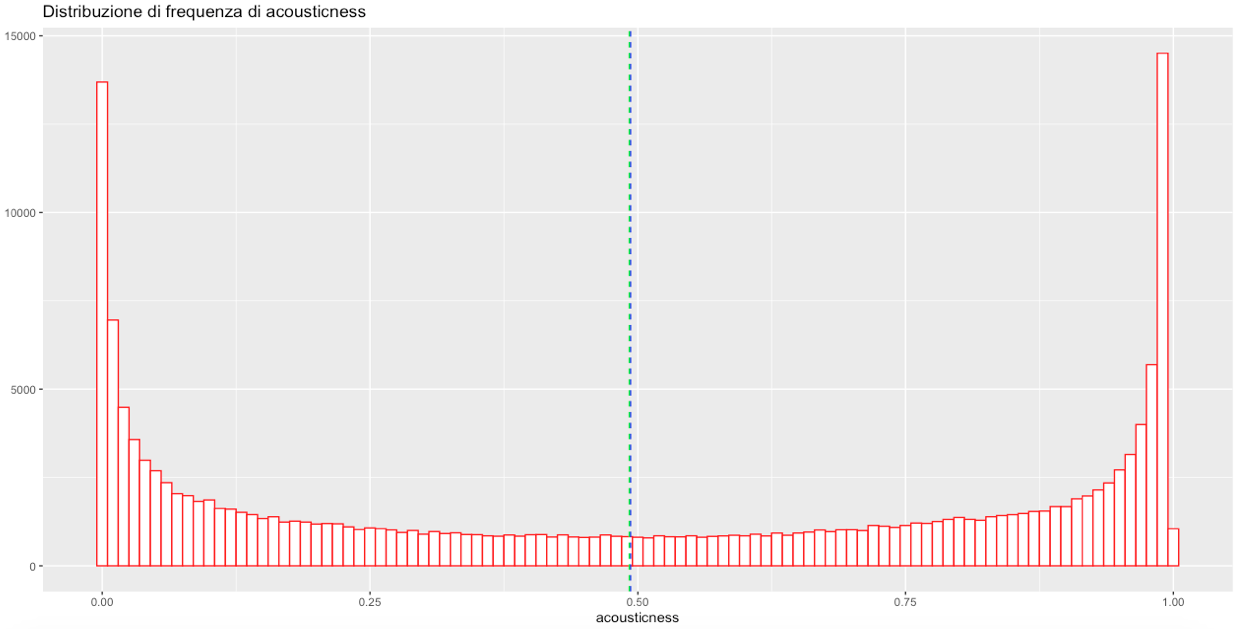
\includegraphics[width=1\linewidth]{fig11.png}
    \label{fig:fig11}
    \caption{Istogramma dell'acusticità. Le linee verticali tratteggiate corrispondono alla media (in blue) e alla mediana (in verde).}
\end{figure}
La forte deviazione dalla condizione Normale è suggerita anche dal grafico \textit{Quantile-Quantile} (Figura \ref{fig:fig12}), specialmente per quanto riguarda le code: quanto minore la somiglianza fra l'andamento dei punti corrispondenti ai quantili empirici e la retta associata alla distribuzione dei quantili teorici normali, tanto maggiore la differenza fra la variabile esaminata e la Gaussiana.
\begin{figure}[H]
    \centering
    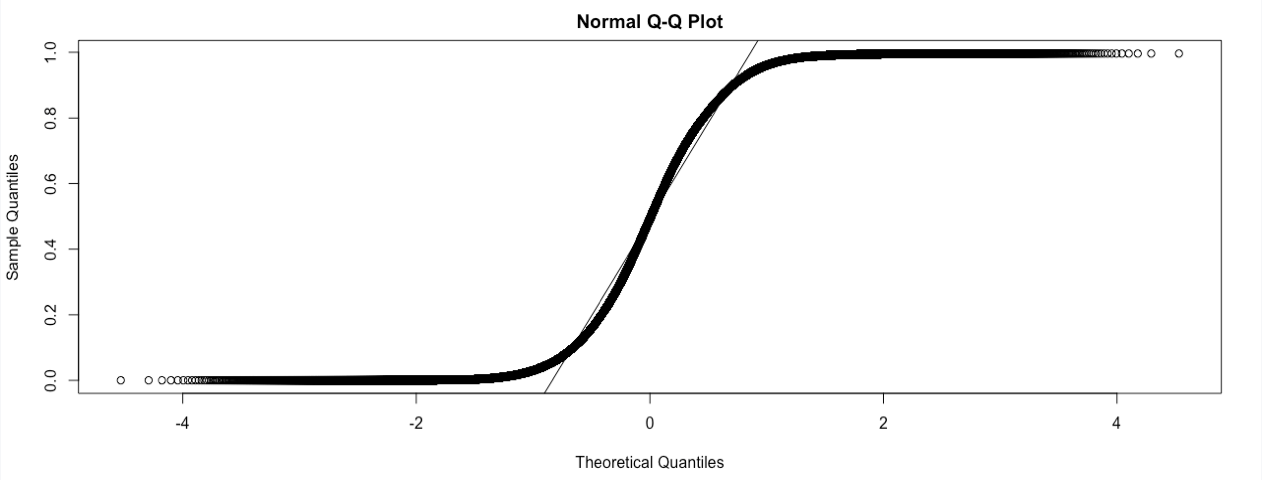
\includegraphics[width=1\linewidth]{fig12.png}
    \label{fig:fig12}
    \caption{Quantile-Quantile Plot per il confronto fra i quantili empirici e i quantili teorici.}
\end{figure}
Infine, con un livello di confidenza al 95\%, è possibile affermare che l'acusticità media sia contenuta nell'intervallo:
\begin{equation}
    (0.491, 0.495)
\end{equation}
Ciò significa che, generalizzando con confidenza al 95\%, le tracce misucali hanno in media una probabilità di essere completamente acustiche inferiore rispetto alla probabilità di includere strumenti elettronici, poichè l'intervallo di confidenza di "acousticness" ha estremo superiore minore di 0.5. 
\subsection*{Variabile \textit{Danceability}}
Le statistiche descrittive sul livello di ballabilità della traccia sono riassunte nella Tabella 2:
{\begin{table}[H]
\centering

\begin{tabular}[t]{lc}
\toprule
\midrule
\textbf{Minimo}&0\\
\textbf{1o Quartile}&0.417\\
\textbf{Mediana}&0.548\\
\textbf{Media}&0.538\\
\textbf{3o Quartile}&0.667\\
\textbf{Massimo}&0.988\\
\textbf{Moda}&0.565\\
\textbf{Coeff. di Variazione}&0.326\\
\bottomrule
\end{tabular}
\caption{Statistiche descrittive calcolate sul livello di ballabilità.}
\end{table}}
La ballabilità dei brani rivela una forma asimmetrica negativa, con un valore dell'indice di asimmetria pari a -0.213. Tale risultato indica che le frequenze più elevate della distribuzione tendono a disporsi su valori elevati di ballabilità, com'è ragionevole supporre, dato che le tracce musicali sono in gran parte concepite per essere accompagnate da qualche forma di ballo. L'allontanamento dalla normalità è molto lieve, di tipo platicurtico (come riscontrato in Figura \ref{fig:fig14}): la curtosi è, infatti, pari a 2.575.\\
\begin{figure}[H]
    \centering
    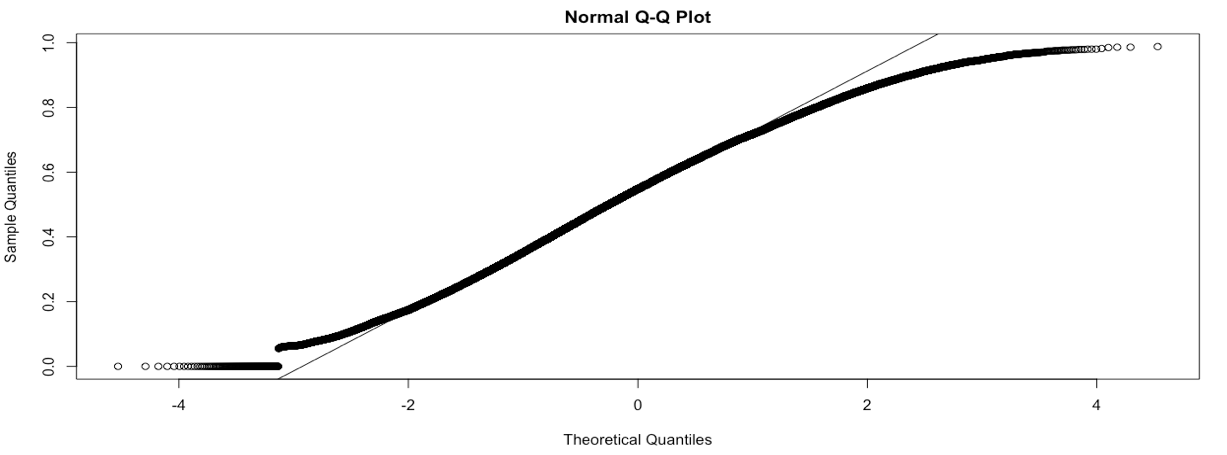
\includegraphics[width=1\linewidth]{fig14.png}
    \label{fig:fig14}
    \caption{Quantile-Quantile Plot per il confronto fra i quantili empirici e i quantili teorici.}
\end{figure}
In Figura \ref{fig:fig13} è visibile la forma della distribuzione della ballabilità.
\begin{figure}[H]
    \centering
    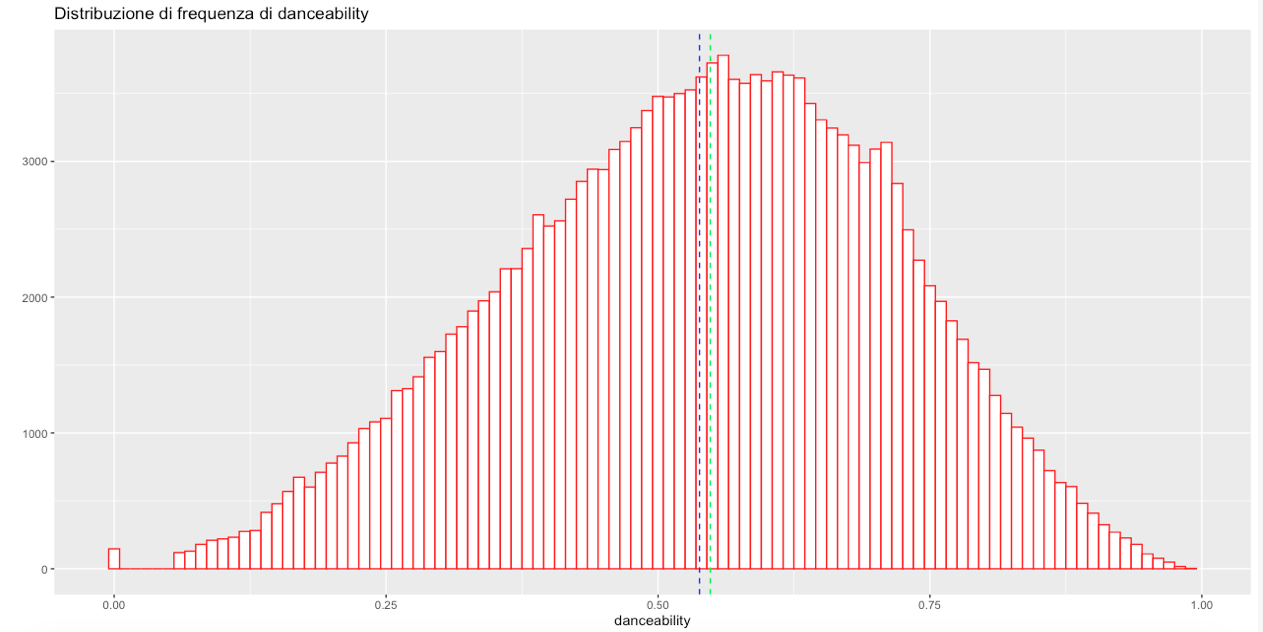
\includegraphics[width=1\linewidth]{fig13.png}
    \label{fig:fig13}
    \caption{Istogramma della ballabilità. Le linee verticali tratteggiate corrispondono alla media (in blue) e alla mediana (in verde).}
\end{figure}
La ballabilità media generale è stimata, con un livello di confidenza del 95\%, nel seguente intervallo:
\begin{equation}
    (0.537, 0.539)
\end{equation}
Si conclude che l'industria discografica preferisce produrre, in media, basi musicali che possano essere più facilmente accompagnate da una danza, ovvero con un livello di {danceability} ben oltre lo 0.5.

\subsection*{Variabile \textit{Instrumentalness}}
Il grado di confidenza con cui si definisce "strumentale" la traccia è, innanzitutto, descritto dalle grandezze in Tabella 3:
{\begin{table}[H]
\centering

\begin{tabular}[t]{lc}
\toprule
\midrule
\textbf{Minimo}&0\\
\textbf{1o Quartile}&0\\
\textbf{Mediana}&0\\
\textbf{Media}&0.162\\
\textbf{3o Quartile}&0.087\\
\textbf{Massimo}&1\\
\textbf{Moda}&0\\
\textbf{Coeff. di Variazione}&1.91\\
\bottomrule
\end{tabular}
\caption{Statistiche descrittive calcolate sul livello di strumentalità.}
\end{table}}
Esso presenta, pertanto, una variabilità nettamente superiore rispetto alle variabili precedentemente esaminate, ed è caratterizzato da una forte asimmetria positiva - misurata pari a 1.682. La forma della distribuzione, descritta da un indice di curtosi superiore a 3 (4.119), è caratterizzata da un allontanamento dalla normalità di tipo leptocurtico: le code tendono ad assottigliarsi, spingengo verso l'alto le frequenze più elevate. Infatti, in Figura \ref{fig:fig15}, soltanto la coda di destra - per la forte asimmetria positiva - si presenta molto lunga ed estremamente sottile. Questa condizione viene riscontrata anche osservando il grafico \textit{Quantile-Quantile} in Figura \ref{fig:fig16}.
\begin{figure}[H]
    \centering
    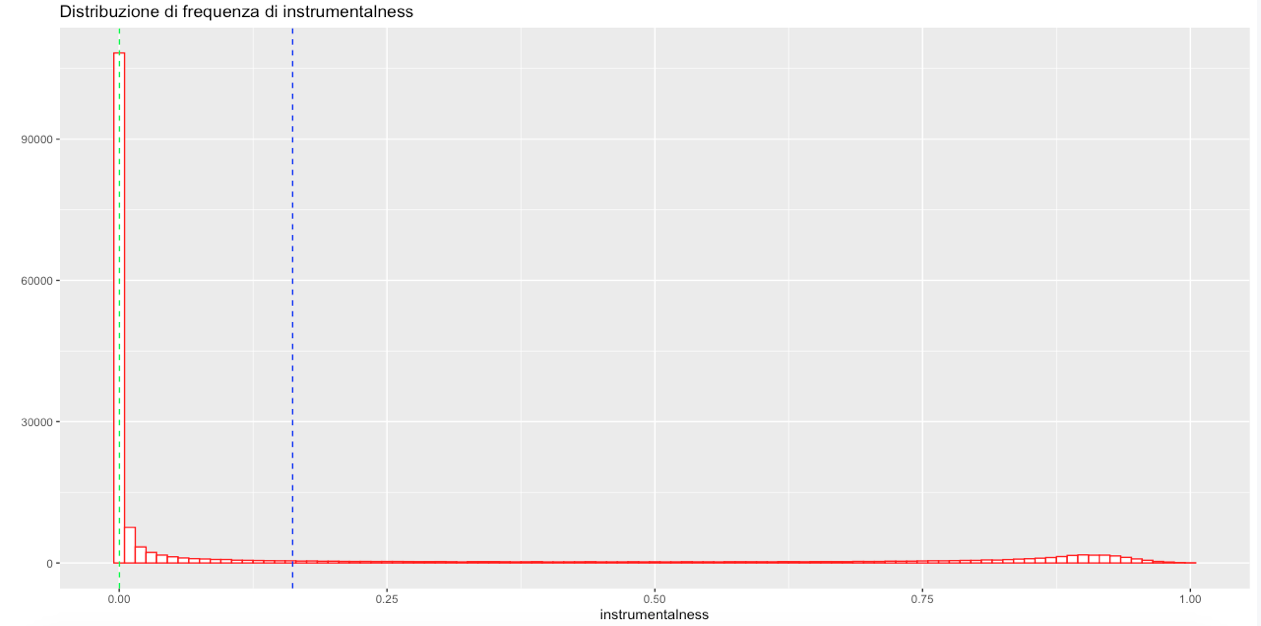
\includegraphics[width=1\linewidth]{fig15.png}
    \label{fig:fig15}
    \caption{Istogramma della \textit{instrumentalness}. Le linee verticali tratteggiate corrispondono alla media (in blue) e alla mediana (in verde).}
\end{figure}. 
\begin{figure}[H]
    \centering
    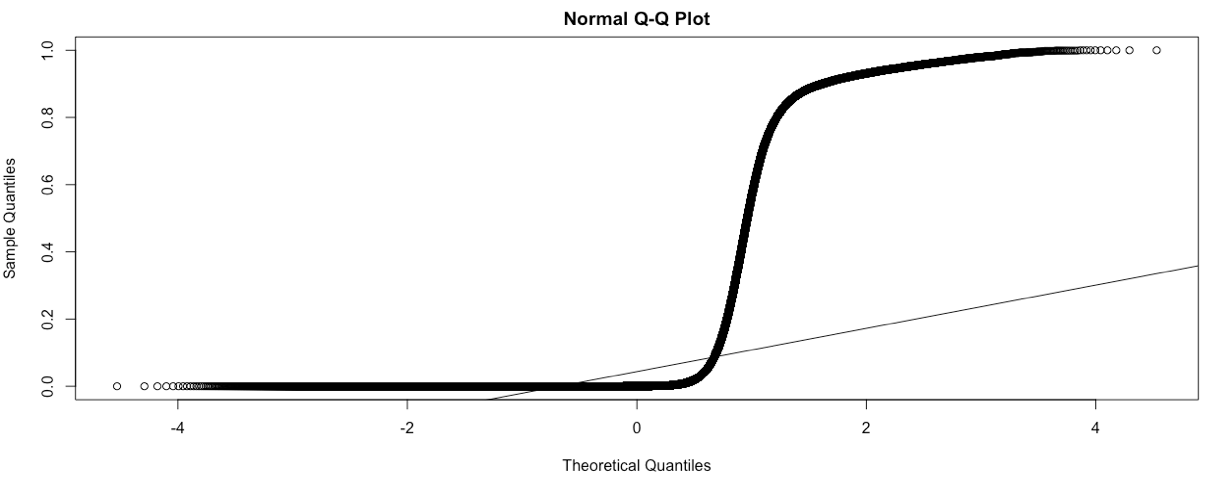
\includegraphics[width=1\linewidth]{fig16.png}
    \label{fig:fig16}
    \caption{Quantile-Quantile Plot per il confronto fra i quantili empirici e i quantili teorici.}
\end{figure}
Infine, la quantità media di contenuto esclusivamente strumentale all'interno delle tracce, con un livello di confidenza del 95\%, viene stimato compreso nel seguente intervallo di confidenza:
\begin{equation}
    (0.16,0.163)
\end{equation}
È quindi ragionevole concludere - con confidenza al 95\% - che, in media, si tenda a produrre brani che contengono al massimo un 16.3\% di parti strumentali.

\subsection*{Variabile \textit{Speechiness}}
Poichè nel paragrafo precedente si è dimostrato come la voce formi elemento tendenzialmente essenziale nella produzione di una traccia, è utile approfondire la variabile che distingue gli elementi vocali in "cantato" e "parlato", con un grado di \textit{speechiness} compreso fra 0 e 1. Le statistiche descrittive di base sono mostrate nella Tabella 4:
{\begin{table}[H]
\centering

\begin{tabular}[t]{lc}
\toprule
\midrule
\textbf{Minimo}&0\\
\textbf{1o Quartile}&0.0349\\
\textbf{Mediana}&0.045\\
\textbf{Media}&0.094\\
\textbf{3o Quartile}&0.075\\
\textbf{Massimo}&0.969\\
\textbf{Moda}&0.0347\\
\textbf{Coeff. di Variazione}&1.594\\
\bottomrule
\end{tabular}
\caption{Statistiche descrittive calcolate sul livello di \textit{speechiness}.}
\end{table}}
La variabilità tende ad essere ancora una volta elevata, e la distribuzione presenta un'asimmetria positiva di gran lunga superiore alle variabili precedenti: 4.236. L'elevatissimo valore di curtosi (22.375) indica che la forma della distribuzione è di tipo leptocurtico, come rilevato riguardo alla "strumentalità", ma con un ulteriore assottigliamento della coda destra (Figura \ref{fig:fig17} e \ref{fig:fig18}).
\begin{figure}[H]
    \centering
    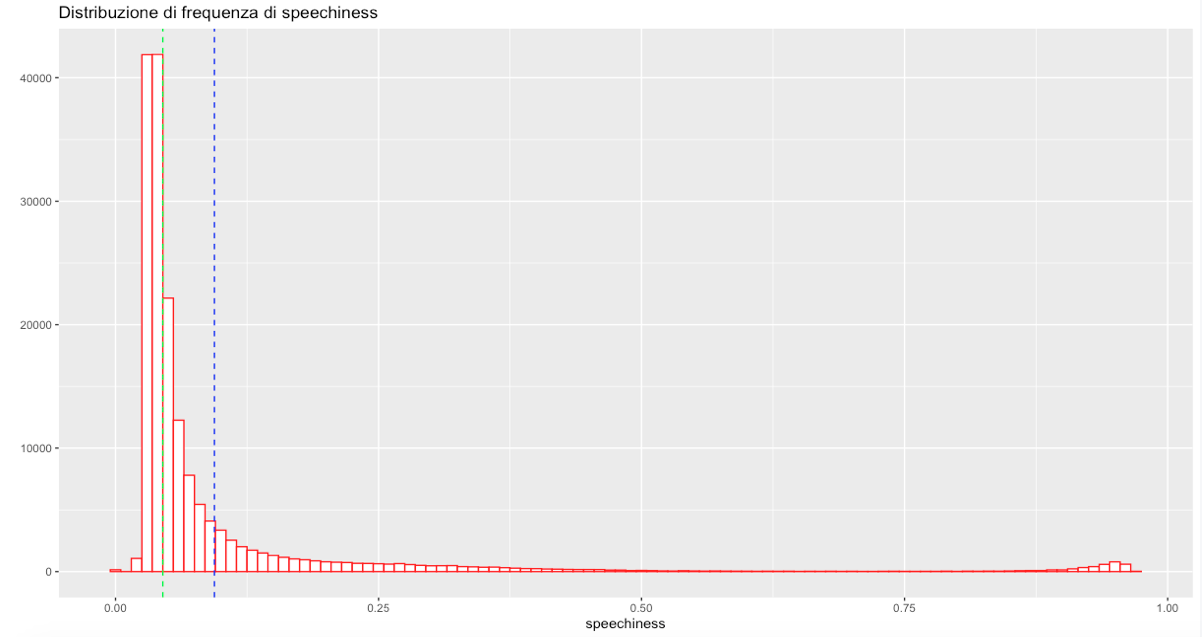
\includegraphics[width=1\linewidth]{fig17.png}
    \label{fig:fig17}
    \caption{Istogramma della \textit{speechiness}. Le linee verticali tratteggiate corrispondono alla media (in blue) e alla mediana (in verde).}
\end{figure}
\begin{figure}[H]
    \centering
    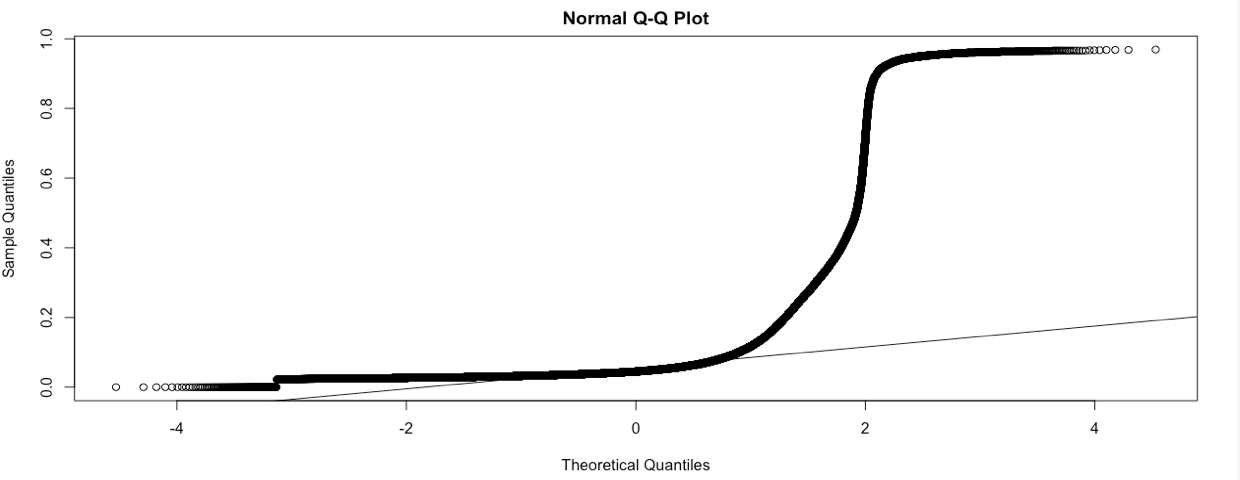
\includegraphics[width=1\linewidth]{fig18.png}
    \label{fig:fig18}
    \caption{Quantile-Quantile Plot per il confronto fra i quantili empirici e i quantili teorici.}
\end{figure}
Queste caratteristiche sono, in altre parole, manifestazione di una generale tendenza a preferire una base vocale cantata, piuttosto che simile ad un discorso, nonostante la grande diffusione di generi musicali come il \textit{rap}. Infatti, la probabilità media di rilevare del parlato all'interno delle canzoni è, comprensibilmente, molto bassa, stimata - con un livello di confidenza del 95\% - all'interno del seguente intervallo:
\begin{equation}
    (0.093, 0.095)
\end{equation}
ovvero tra il 9.3\% e il 9.5\%.

\subsection*{Variabile \textit{Liveness}}
Un altro carattere quantitativo interessante consiste nella probabilità che la traccia sia stata registrata durante un'esibizione dal vivo. Le statistiche descrittive sono riportate in Tabella 5:
{\begin{table}[H]
\centering

\begin{tabular}[t]{lc}
\toprule
\midrule
\textbf{Minimo}&0\\
\textbf{1o Quartile}&0.0984\\
\textbf{Mediana}&0.135\\
\textbf{Media}&0.207\\
\textbf{3o Quartile}&0.263\\
\textbf{Massimo}&1\\
\textbf{Moda}&0.111\\
\textbf{Coeff. di Variazione}&0.855\\
\bottomrule
\end{tabular}
\caption{Statistiche descrittive calcolate sul livello di \textit{liveness}.}
\end{table}}
La distribuzione è positivamente asimmetrica, con un indice pari a 2.146, e leptocurtica ($\frac{m_4}{m_2^{2}}=7.916$). La sua variabilità è moderata. In Figura \ref{fig:fig19}, è possibile notare la sottile coda di destra, specialmente per valori maggiori di 0.5, e l'elevata frequenza delle probabilità più ridotte, in un intervallo compreso fra 0 e, circa, 0.375. L'allontanamento dalla condizione di normalità è perfettamente descritto nel grafico \textit{Quantile-Quantile} (Figura \ref{fig:fig20}): anche qui, come nei due casi precedenti, i quantili empirici relativi alla coda destra sono estremamente distanti da quelli teorici.
\begin{figure}[H]
    \centering
    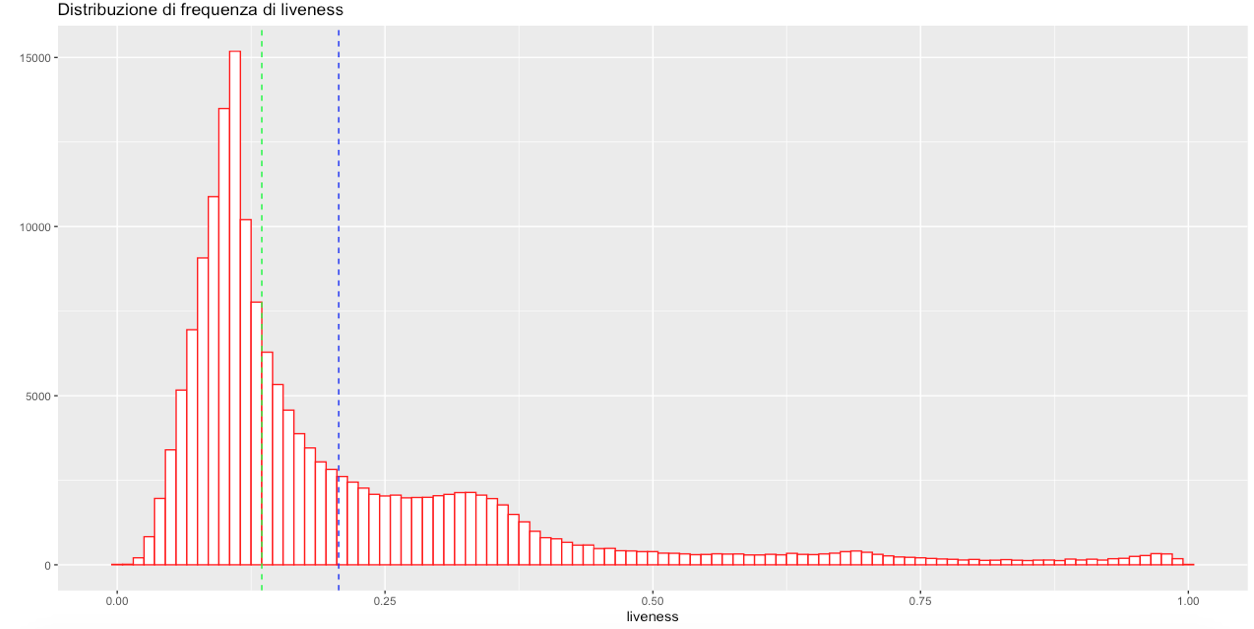
\includegraphics[width=1\linewidth]{fig19.png}
    \label{fig:fig19}
    \caption{Istogramma della \textit{liveness}. Le linee verticali tratteggiate corrispondono alla media (in blue) e alla mediana (in verde).}
\end{figure}
\begin{figure}[H]
    \centering
    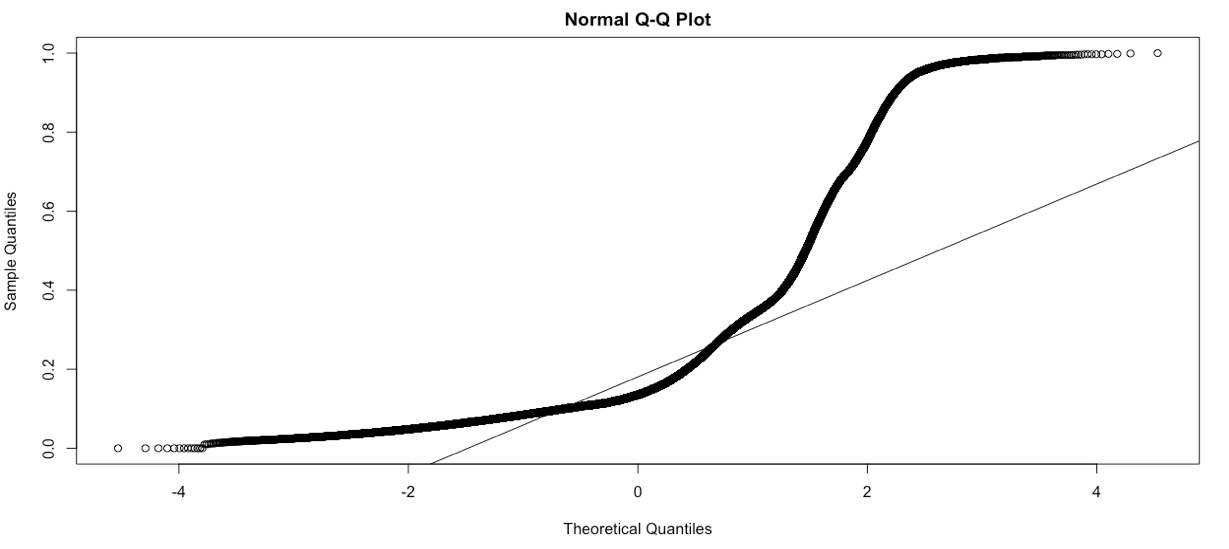
\includegraphics[width=1\linewidth]{fig20.png}
    \label{fig:fig20}
    \caption{Quantile-Quantile Plot per il confronto fra i quantili empirici e i quantili teorici.}
\end{figure}
Infine, è possibile affermare, con confidenza al 95\%, che la probabilità media che la traccia sia stata registrata dal vivo sia compresa nell'intervallo
\begin{equation}
    (0.206, 0.208)
\end{equation}

\subsection*{Variabile \textit{Valence}}
La variabile che registra la positività percepita durante l'ascolto del brano è caratterizzata dalle seguenti  statistiche di base (Tabella 6):
{\begin{table}[H]
\centering

\begin{tabular}[t]{lc}
\toprule
\midrule
\textbf{Minimo}&0\\
\textbf{1o Quartile}&0.322\\
\textbf{Mediana}&0.544\\
\textbf{Media}&0.532\\
\textbf{3o Quartile}&0.749\\
\textbf{Massimo}&1\\
\textbf{Moda}&0.961\\
\textbf{Coeff. di Variazione}&0.493\\
\bottomrule
\end{tabular}
\caption{Statistiche descrittive calcolate sul livello di positività.}
\end{table}}
La distribuzione presenta una leggera asimmetria negativa (-0.124) e una forma platicurtica - la curtosi è 1.949 -, come osservato in Figura \ref{fig:fig21}. 
\begin{figure}[H]
    \centering
    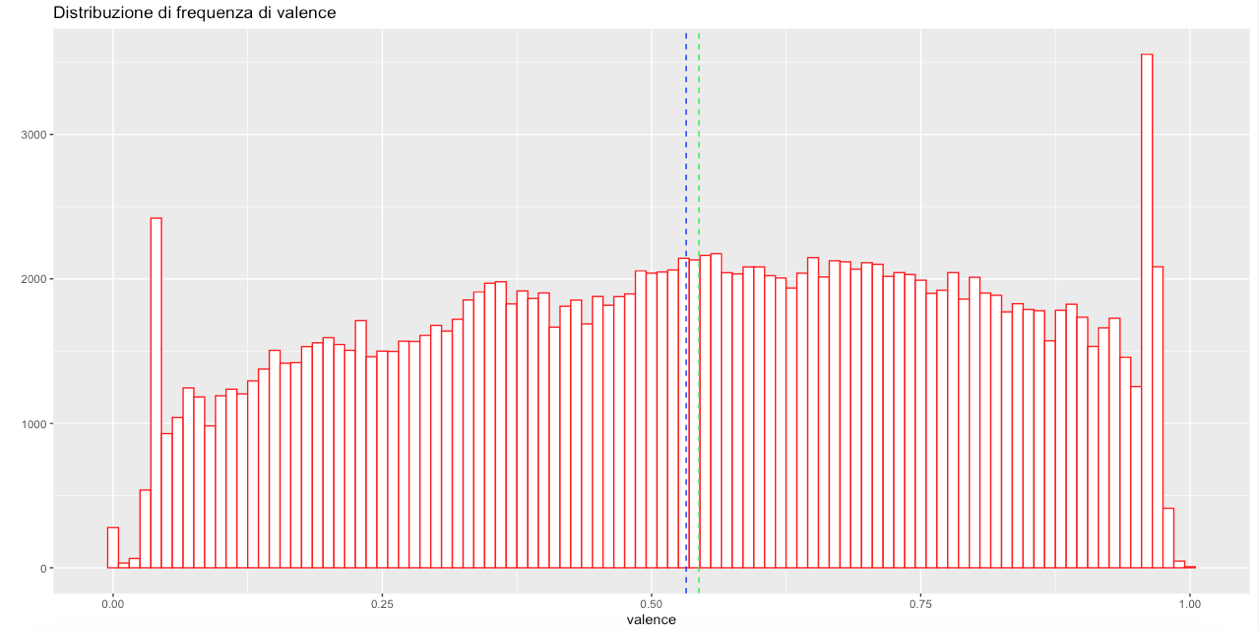
\includegraphics[width=1\linewidth]{fig21.png}
    \label{fig:fig21}
    \caption{Istogramma della positività trasmessa dal brano. Le linee verticali tratteggiate corrispondono alla media (in blue) e alla mediana (in verde).}
\end{figure}
Le code spesse deformano la tipica forma a campana verso una densità visibilmente più piatta. Questa anomalia è riscontrabile in Figura \ref{fig:fig22}.
\begin{figure}[H]
    \centering
    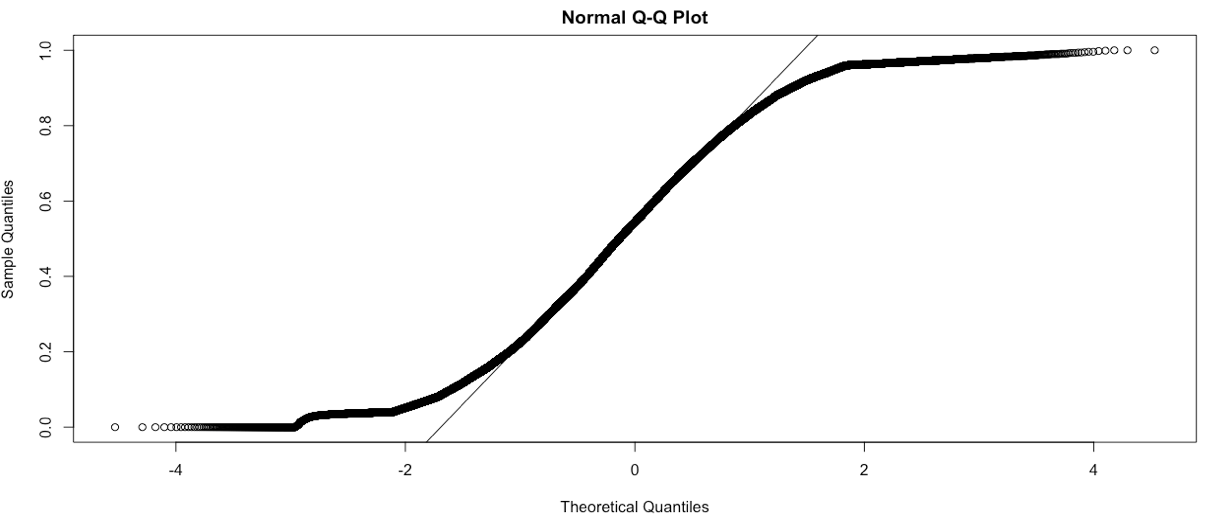
\includegraphics[width=1\linewidth]{fig22.png}
    \label{fig:fig22}
    \caption{Quantile-Quantile Plot per il confronto fra i quantili empirici e i quantili teorici.}
\end{figure}
Il livello emotivo, pertanto, si distribuisce in maniera bilanciata: la produzione musicale, nelle proprie numerose declinazioni di genere, è in grado di esprime qualsiasi tipo di stato d'animo, dal più negativo - quando \textit{valence} è nulla - al più positivo - quando la colonna assume valore 1, senza essere dominata da nessuna delle due polarità. Tuttavia, con confidenza al 95\%, è possibile affermare che l'industria discografica propenda leggermente verso un sentimento più positivo, poiché il livello emotivo medio è stimato all'interno dell'intervallo
\begin{equation}
    (0.531, 0.533)
\end{equation}
\\
Si è proceduto, poi, a verificare l'esistenza di qualche tipo di connessione statistica fra il livello emotivo e altre variabili qualitative. Innanzitutto, si è deciso di studiare il legame fra il decennio di pubblicazione e la positività trasmessa, per estrarre evidenze sul fatto che i contenuti musicali risentano del periodo storico non solo da un punto di vista stilistico, ma anche da un punto di vista dei sentimenti espressi. Pertanto, è stato eseguito un test del Chi-quadrato sulla relazione fra \textit{Valence} e \textit{Decade}, con 1 grado di libertà, supponendo una reciproca indipendenza fra le varie decadi. Fissato un livello di significatività del 5\%, s'ottiene un \textit{pvalue} inferiore alla soglia, rifiutando l'ipotesi di indipendenza. Viene anche rifiutata l'ipotesi di uguaglianza dei livelli emotivi medi per ogni decennio, tramite test ANOVA con $\alpha=0.05$ e 10 gradi di libertà, confermando ulteriormente l'esistenza di una relazione fra i due fenomeni. In Figura \ref{fig:fig23}, è possibile distinguere le differenti distribuzioni della positività per gruppo. 
\begin{figure}[H]
    \centering
    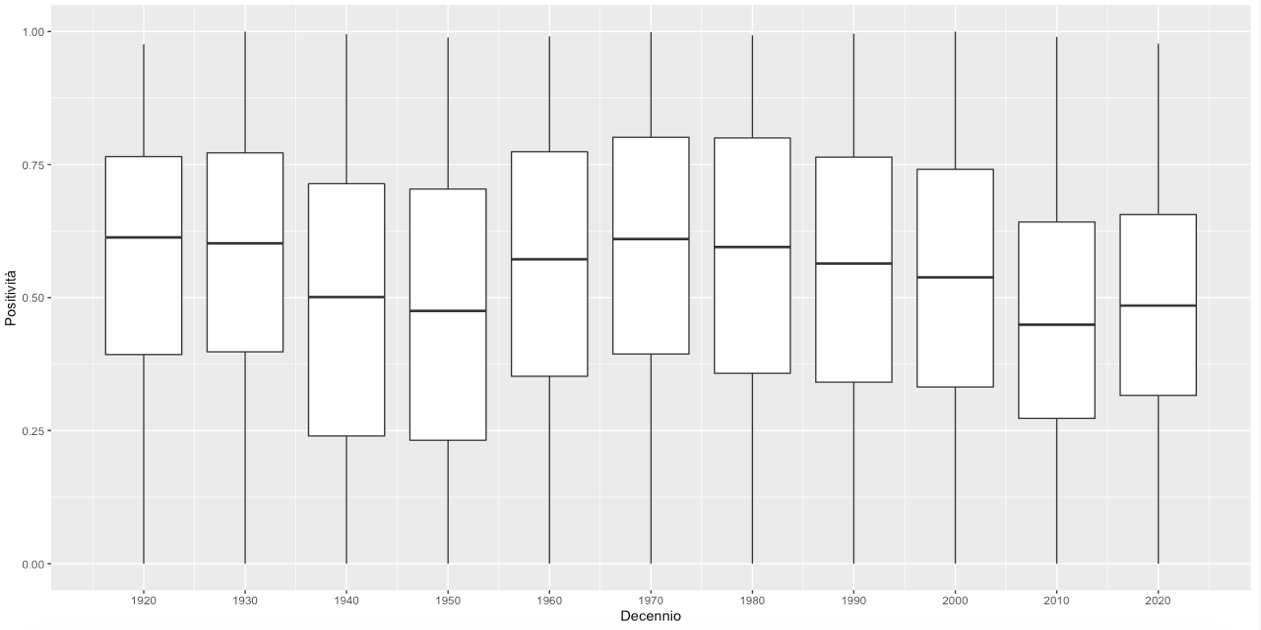
\includegraphics[width=1 \linewidth]{fig23.png}
    \label{fig:fig23}
    \caption{\textit{BoxPlot} condizionati per la visualizzazione delle distribuzioni condizionate di positività in base al decennio esaminato.}
\end{figure}
Nella stessa maniera, vengono esaminate le dipendenze della positività rispetto alla tonalità e alla chiave del brano, ipotizzando che gli elementi tecnici di base possano influenzare il sentimento della traccia finale. In entrambi i casi, l'ipotesi di indipendenza viene rifiutata tramite calcolo dell'indice di connessione $\chi^2$ con livello di significatività 0.05, e così anche l'ipotesi di uguaglianza delle medie di \textit{Valence} rispetto a entrambi i fattori condizionanti - test ANOVA -, sempre con confidenza al 95\%.

\subsection*{Variabile \textit{Popularity}}
La popolarità è associata alle seguenti statistiche (Tabella 6):
{\begin{table}[H]
\centering
\begin{tabular}[t]{lc}
\toprule
\midrule
\textbf{Minimo}&0\\
\textbf{1o Quartile}&12\\
\textbf{Mediana}&33\\
\textbf{Media}&31.56\\
\textbf{3o Quartile}&48\\
\textbf{Massimo}&100\\
\textbf{Moda}&0\\
\textbf{Coeff. di Variazione}&0.684\\
\bottomrule
\end{tabular}
\caption{Statistiche descrittive calcolate sul livello di popolarità.}
\end{table}}
La moda viene individuata in corrispondenza di 0: il grado di popolarità su \textit{Spotify} più diffuso all'interno del campione esaminato è quello nullo, coprendo addirittura fino al 16.1\% delle osservazioni totali. La variabilità è bassa e la distribuzione rivela un discreto indice di asimmetria negativo, pari a -0.021, e un forma moderatamente platicurtica (Figura \ref{fig:fig25}), con curtosi uguale a 1.985. Osservando la Figura \ref{fig:fig24}, è possibile notare, senza considerare il valore di moda, come le misure più frequenti siano concentrate nell'intervallo 25-50.
\begin{figure}[H]
    \centering
    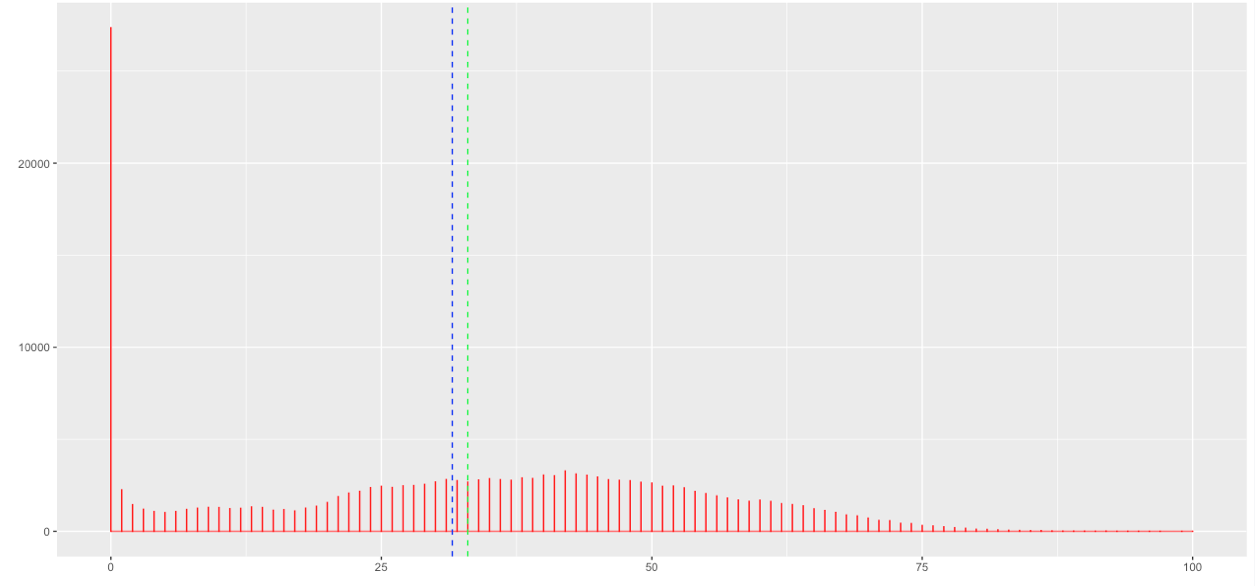
\includegraphics[width=1\linewidth]{fig24.png}
    \label{fig:fig24}
    \caption{Istogramma della popolarità. Le linee verticali tratteggiate corrispondono alla media (in blue) e alla mediana (in verde).}
\end{figure}
\begin{figure}[H]
    \centering
    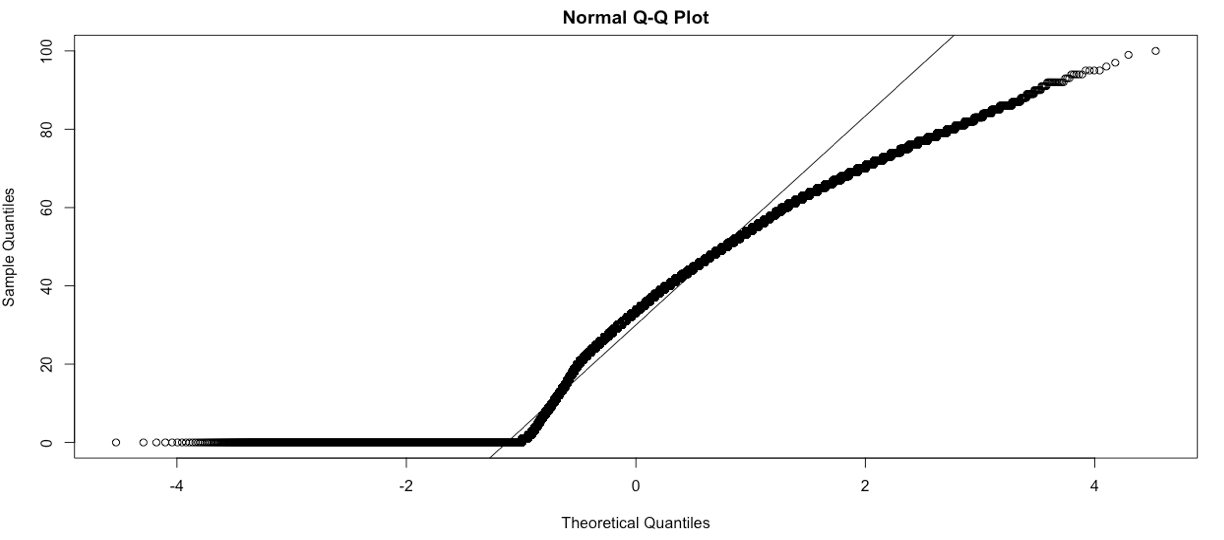
\includegraphics[width=1\linewidth]{fig25.png}
    \label{fig:fig25}
    \caption{Quantile-Quantile Plot per il confronto fra i quantili empirici e i quantili teorici.}
\end{figure}
\subsection{Correlazioni lineari}
Successivamente, sono stati stimati i coefficienti di correlazione di Pearson per tutte le possibili coppie di variabili quantitative, effettuando il corrispettivo test con livello di confidenza fissato al 95\%, per valutare la significatività statistica dei valori $\rho$. Il grado di reciproca dipendenza lineare fra i vari caratteri è visibile in Figura \ref{fig:fig26}.
\begin{figure}[H]
    \centering
    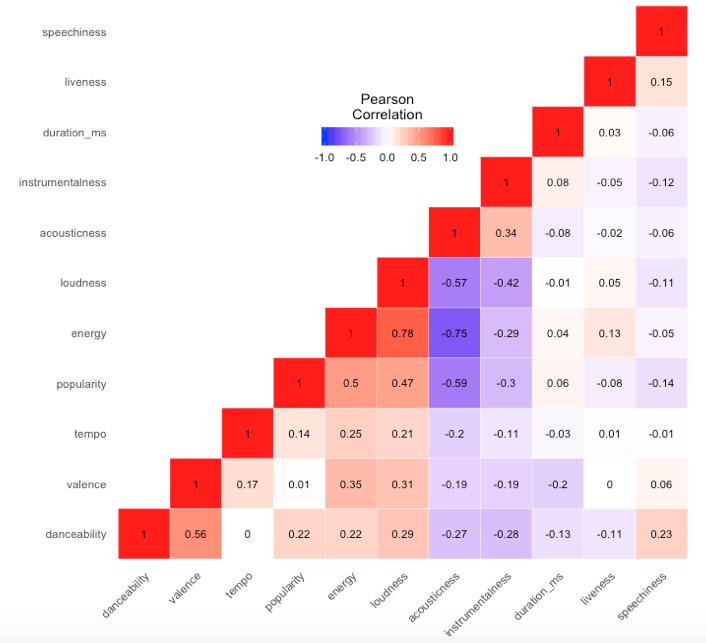
\includegraphics[width=1\linewidth]{fig26.png}
    \label{fig:fig26}
    \caption{\textit{Heatmap} per la visualizzazione dei coefficienti di correlazione lineare di Pearson fra tutte le variabili quantitative.}
\end{figure}
L'unica correlazione lineare statisticamente non significativa ad un livello di confidenza del 95\% viene riscontrata fra \textit{liveness} e positività: il \textit{pvalue} è 0.86.\\
I valori $\rho$ più rilevanti possono essere riscontrati fra le seguenti coppie di fenomeni:
\begin{itemize}
    \item energia e volume: $\rho=0.78$ 
    \item energia e "acusticità": $\rho=-0.75$
    \item popolarità e "acusticità: $\rho=-0.59$, per cui i brani con strumenti elettronici attrarrebbero maggiori ascolti
    \item volume e "acusticità": $\rho=-0.57$, per cui all'assenza di strumenti elettronici si associa un minor livello di decibel
    \item ballabilità e \textit{valence}: $\rho=0.56$, per cui maggiore la positività percepita dall'ascolto di un brano, maggiore la facilità ad associargli una danza, e viceversa. 
\end{itemize}
In fase di costruzione di un modello di regressione lineare, sarà necessario valutare queste collinearità fra le colonne della matrice del disegno, poiché potrebbero penalizzare la corretta stima dei coefficienti di regressione.
%------------------------------------------------
\section{Regressione semplice}

%------------------------------------------------
\section{Regressione multipla}
\subsection{Previsione di \textit{Popularity}}
\subsection{Previsione di \textit{Valence}}
%------------------------------------------------
\section{Conclusioni}

%------------------------------------------------
\section*{Codice}
L'intero codice, implementato con linguaggio \texttt{R}, è disponibile al link: \href{https://github.com/RCrvro/Foundation-of-Prob.-and-Stat.---Final-Project/blob/master/codice.R}{\texttt{github.com/RCrvro/codice.R}}.
%----------------------------------------------------------------------------------------

\end{document}

